\documentclass[12pt]{article}
\usepackage[top=1in, bottom=1.25in, left=1.25in, right=1.25in]{geometry}
\usepackage{setspace} % For line spacing e.g. \onehalfspacing
\usepackage{graphicx}
\usepackage{hyperref}
\usepackage{listings}
\usepackage{amsmath}
\usepackage{algorithm}
\usepackage{algpseudocode}
\usepackage{pdfpages}

\title{Comp 6231 -- Assignment 2\\RMI}
\author{Saman Saadi Alekasir\\Student ID: 40009949}
\date{November 5, 2017}
\onehalfspacing

\begin{document}
\begin{titlepage}
\clearpage
\pagenumbering{roman}
\maketitle
\thispagestyle{empty}
\end{titlepage}
\pagenumbering{arabic}

\section{Adopting to New Requirements}
I decided to separate business logic from communication technology. In other words, My $Campus$ class which is responsible to implement campus servers functionality contain only business logic of the servers. Both RMI and CORBA use this class for handling user requests. Due to checked exceptions in Java, It wasn't feasible to write one interface for both of them. Because they have different classes for exception handling.
\par Because of this separation I can run both RMI and CORBA with the same functionality. I defined a variable to determine communication technology. At the moment I only support RMI and CORBA and hopefully with a little changes I can support web services also. You can see a rough class diagram in figure \ref{fig:class_diagram}.

\begin{figure}
\caption{Rough class diagram}
\centering
\label{fig:class_diagram}
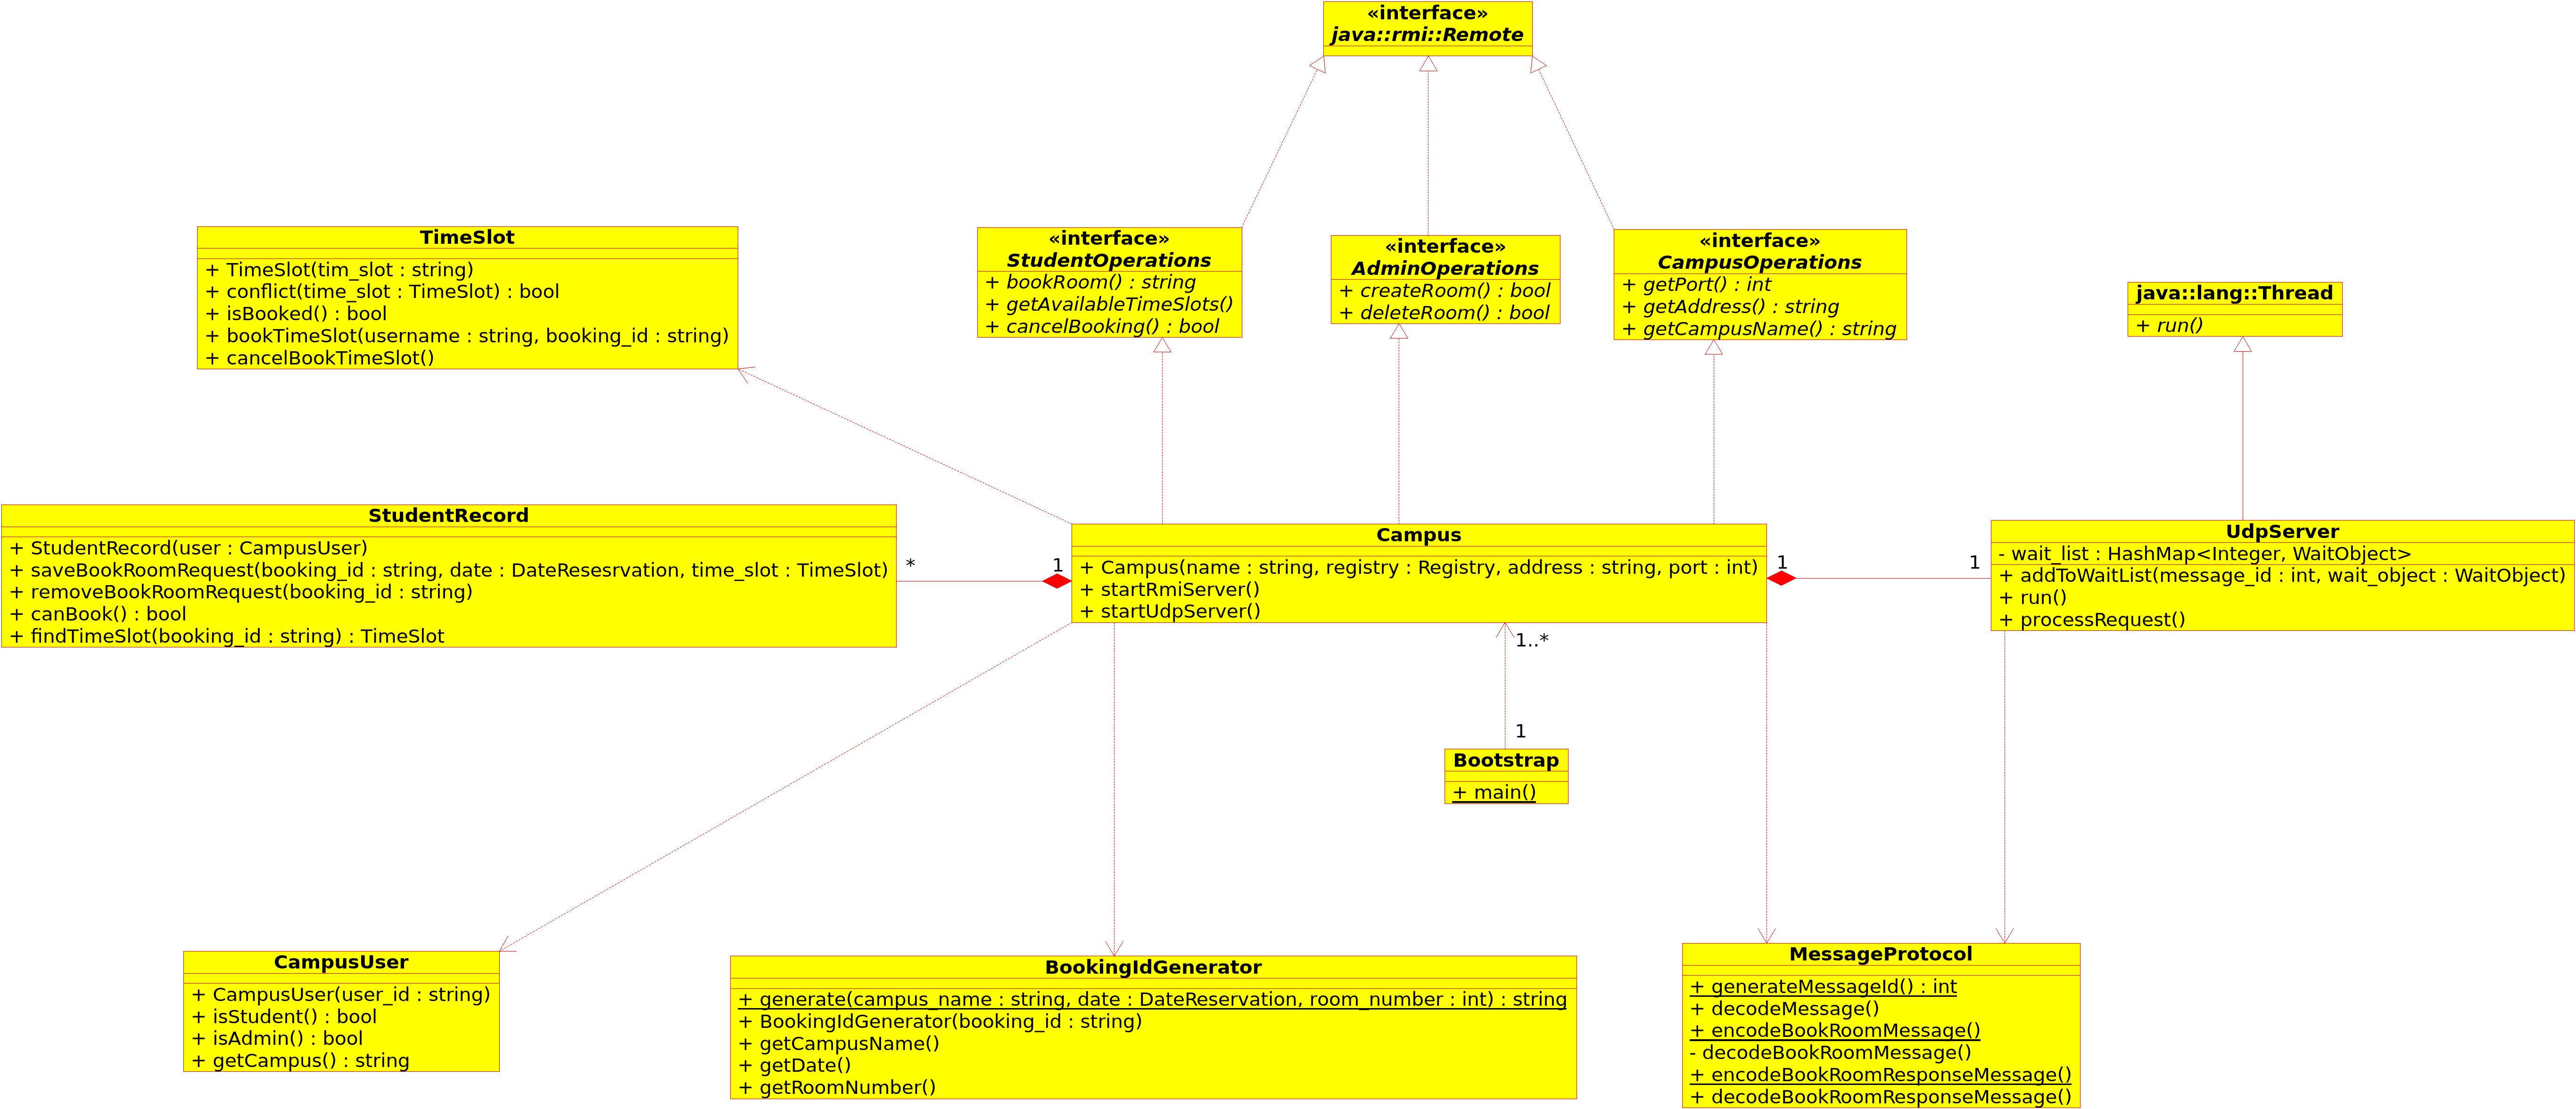
\includegraphics[width=\linewidth]{img/class_diagram.png}
\end{figure}

\section{Implementing the New Functionality}

Since changing room reservation should be a transaction, first I try to book the new time slot and then remove the previous time slot. By doing that I have the concept of a transaction. The only problem is the user now can book more than 3 time slots. So I allow the user temporary book more than 3 time slots and after the transaction completed the amount of booked time slots per user should be at most 3.

\section{Synchronization}
According to Java SE 8 documentation \cite{hashmap}: "if multiple threads access a hash map concurrently, and at least one of the threads modifies the map structurally, it must be synchronized externally. (A structural modification is any operation that adds or deletes one or more mappings; merely changing the value associated with a key that an instance already contains is not a structural modification.). This is typically accomplished by synchronizing on some object that naturally encapsulates the map". So it is not safe to use $HashMap.get$ when another thread try to change $HashMap$'s structure \cite{hashmap-multithread-get}. I should also mention $HashMap$ is not thread-safe for different keys \cite{hashmap-multithread-different-keys}.
\subsection{Main Database}
I designed three types of object locks for handling $HashMap$ database for multi-threaded environment. One locks the first key (date of reservation), the other locks the second key (room number) and the third locks a list of time slots for a specific date and room number.
\par I've noticed $createRoom$ is similar to $deleteRoom$ but some parts are different. For handling that I design a system which is used in event-handling systems. I define a private method named $traverseDb$ which handles all synchronization when we traverse the database and call some abstract methods for handling different implementation between $createRoom$ and $deleteRoom$ operations. In other words, those methods should implement abstract class methods define in listing \ref{lst:DbOperations}. I removed the arguments and the return value for simplicity. As you can see all of them are thread-safe (unless we try to access another database or container). In other words, $createRoom$ and $deleteRoom$ should only implement these thread-safe callbacks. Handling the synchronization is done in $traverseDb$ method.

\begin{lstlisting}[language=java,label={lst:DbOperations},caption={DbOperations abstract class},numbers=left]
private abstract class DbOperations
{
  //All the following methods 
  //are thread-safe for campus time slots database
  public abstract onNullValue();
  public abstract onNullSubValue();
  public abstract void onSubValue();
}
\end{lstlisting}

\par You can see a snippet of $traverseDb$ method implementation in listing \ref{lst:traverse_db}. It is important to put lines 2 - 8 in a $synchronization$ block. In $createRoom$ method it implements $onNullValue$ by creating a new $HashMap$ for room number and list of time slots. If more than one thread try to execute it, each of them has their own new $HashMap$ of room number and list of time slots which is not correct because one of those two threads has stale value.

\begin{lstlisting}[language=java,label={lst:traverse_db},caption={Snippet from traverseDb method},numbers=left]
synchronized (date_db_lock) {
  val = db.get(date);
  if (val == null)
  {
    val = db_ops.onNullValue();
    if (val == null)
      return;
    db.put(date, val);
  }
}		
\end{lstlisting}

\par According to problem statement, we need to update student record when we delete a time slot which that user has booked. I create a thread for every time slot which is booked by a user from another campus which is responsible to get notification about the status of student record's update from another campus. At the end of method I'm going to wait for all created threads to finish their job.

\subsection{Student Database}
This database store the records of a particular student reservation and make sure it does not exceed 3 times per week. I follow the same pattern as main database. I've noticed $bookRoom$ and $cancelBooking$ have a lot in common. So I created a private method named $traverseStudentDb$ which handles traversing student database and calls some callbacks which are implemented differently in $bookRoom$ and $cancelBooking$ methods. You can see the abstract class which both methods should implement in listing \ref{lst:traverse_student_db}. All these methods are thread-safe, unless we want to access another database or container.

\begin{lstlisting}[language=java,label={lst:traverse_student_db},caption={UserDbOperations Abstract Class},numbers=left]
private abstract class UserDbOperations
{
  //All the following methods are tread-safe for user database
  public abstract boolean onUserBelongHere(record);
  public abstract StudentRecord onNullUserRecord(user);
  public abstract boolean onOperationOnThisCampus(time_slots);
  public abstract void onOperationOnOtherCampus(message_id); 
  public abstract void onPostUserBelongHere(record);
  public abstract ArrayList<TimeSlot> findTimeSlots();
}
\end{lstlisting}

\par I also try to lock student's record during the transaction. For example when user wants to book a room on another campus, the student record should be locked until we receive answer through UDP communication. When the campus send booking request to another campus, it create a $WaitObject$ object and then calls its $wait$ method. It's the responsibility of UDP server to notify it that its response has arrived.

\subsection{Container Synchronization}
According to $ArrayList$ documentation \cite{ArrayList}: "If multiple threads access an ArrayList instance concurrently, and at least one of the threads modifies the list structurally, it must be synchronized externally. (A structural modification is any operation that adds or deletes one or more elements, or explicitly resizes the backing array; merely setting the value of an element is not a structural modification.) This is typically accomplished by synchronizing on some object that naturally encapsulates the list.". So I need to synchronize accessing $ArrayList$ (or other collections) when I want to access an element or traverse it. According to $Collections$ documentation \cite{Collections}: "It is imperative that the user manually synchronize on the returned list when iterating over it (see listing \ref{lst:collections-sync})".

\begin{lstlisting}[language=java,label={lst:collections-sync},caption={Collections Synchronization},numbers=left]
List list = Collections.synchronizedList(new ArrayList());
    ...
synchronized (list) {
  Iterator i = list.iterator(); // Must be in synchronized block
  while (i.hasNext())
    foo(i.next());
}
\end{lstlisting}

\subsection{Socket Synchronization}
It is safe to have two threads which one of them read from socket and the other write into it concurrently \cite{socket-full-duplex}. I only have one reader thread so I don't need to do synchronization here. But I can have multiple thread for writing into socket so synchronization is necessary.

\section{Testing Scenario}
I've changed the client side classes like the server side. So my client classes don't have any information about the underlying communication technology. So it was easy to use previous assignment unit tests. I also write some new unit tests for testing the new functionality in this assignment.
\section{Conclusion}
Since in three assignments we have the same functionality but different technology, I thought it would be better to separate the core implementation from communication technology in this assignment. So I have a two layer architecture. The main layer is responsible for providing services for communication layer which can be CORBA or RMI.
\bibliographystyle{unsrt}
\bibliography{bibs/websites}
\end{document}
